\documentclass[aspectratio=169,12pt,t]{beamer}

% --- Theme: Metropolis (modern, clean) ---
\usetheme[progressbar=frametitle,numbering=fraction,block=fill]{metropolis}

% --- Fira Sans font (install texlive-fonts-extra if missing) ---
\IfFileExists{FiraSans.sty}{\usepackage[sfdefault]{FiraSans}}{}

% --- Light background with warm accent ---
\definecolor{mDarkTeal}{RGB}{35,55,59}
\definecolor{mLightBrown}{RGB}{235,228,216}
\definecolor{mAccent}{RGB}{140,70,20}

\setbeamercolor{normal text}{fg=mDarkTeal,bg=white}
\setbeamercolor{alerted text}{fg=mAccent}
\setbeamercolor{frametitle}{bg=mDarkTeal,fg=white}
\setbeamercolor{progress bar}{fg=mAccent,bg=mLightBrown}
\setbeamercolor{title separator}{fg=mAccent}
\setbeamercolor{progress bar in head/foot}{fg=mAccent,bg=mLightBrown}
\setbeamercolor{progress bar in section page}{fg=mAccent,bg=mLightBrown}

% --- Packages ---
\usepackage[utf8]{inputenc}
\usepackage{amsmath,amssymb,amsthm}
\usepackage{mathrsfs}
\usepackage{tikz}
\usetikzlibrary{arrows.meta,positioning,calc,decorations.pathreplacing,shapes,patterns}
\usepackage{pgfplots}
\pgfplotsset{compat=1.18}

% --- TikZ diagram styles (shared across the series) ---
\tikzset{
  axisln/.style={-{Stealth[length=2.6mm]}, line width=0.8pt, gray!75},
  curveln/.style={line width=1.6pt, line cap=round, line join=round},
  projln/.style={dash pattern=on 2.6pt off 2pt, line width=0.7pt},
  guide/.style={-{Stealth[length=2.6mm,width=2.2mm]}, line width=1.1pt},
}
% point marker with a white halo: \dotpt{color}{(coord)}
\newcommand{\dotpt}[2]{%
  \fill[white] #2 circle (3.6pt);
  \fill[#1] #2 circle (2.4pt);
}
% open point marker: \opendotpt{color}{(coord)}
\newcommand{\opendotpt}[2]{%
  \fill[white] #2 circle (3.6pt);
  \draw[#1, line width=1pt] #2 circle (2.4pt);
}

% --- Semi-transparent white highlight for text on top of background images ---
\usepackage[most]{tcolorbox}

% Inline highlight: \hl{short text}
\newtcbox{\hl}{%
  nobeforeafter, tcbox raise base,
  colback=white, opacityback=0.6,
  colframe=white, opacityframe=0,
  sharp corners, boxsep=2pt, left=3pt, right=3pt, top=2pt, bottom=2pt%
}

% Block highlight: \begin{hlbox} ... \end{hlbox}  (multi-line, paragraphs, itemize)
% Optional argument accepts any tcolorbox key, e.g. [width=0.6\linewidth]
\newtcolorbox{hlbox}[1][]{%
  enhanced, breakable,
  colback=white, opacityback=0.6,
  colframe=white, opacityframe=0,
  boxsep=3pt, left=6pt, right=6pt, top=4pt, bottom=4pt,
  sharp corners,
  {#1}%
}

% --- Custom colors for content types ---
\definecolor{defcolor}{RGB}{25,85,120}
\definecolor{thmcolor}{RGB}{140,35,35}
\definecolor{proofcolor}{RGB}{35,100,50}
\definecolor{excolor}{RGB}{140,75,10}
\definecolor{remcolor}{RGB}{90,90,90}

% --- Beamer blocks for mathematical content types (semi-transparent) ---
\tcbset{hlblockbase/.style={
  enhanced, breakable,
  coltitle=white, fonttitle=\bfseries,
  opacitybacktitle=0.8, opacityback=0.6,
  opacityframe=0,
  sharp corners,
  boxsep=1pt, left=5pt, right=5pt, top=2pt, bottom=2pt,
  toptitle=1pt, bottomtitle=1pt
}}

\newtcolorbox{defblock}[1]{hlblockbase, title={#1},
  colbacktitle=defcolor, colback=defcolor!15, colframe=defcolor}
\newtcolorbox{thmblock}[1]{hlblockbase, title={#1},
  colbacktitle=thmcolor, colback=thmcolor!15, colframe=thmcolor}
\newtcolorbox{proofblock}[1]{hlblockbase, title={#1},
  colbacktitle=proofcolor, colback=proofcolor!15, colframe=proofcolor}
\newtcolorbox{exblock}[1]{hlblockbase, title={#1},
  colbacktitle=excolor, colback=excolor!15, colframe=excolor}
\newtcolorbox{remblock}[1]{hlblockbase, title={#1},
  colbacktitle=remcolor, colback=remcolor!15, colframe=remcolor}

% --- Metadata ---
\title{Chapter 5: Differentiation}
\subtitle{Section: L'Hospital's Rule}
\author{Based on Walter Rudin's \emph{Principles of Mathematical Analysis}}
\date{}

\begin{document}

{
\usebackgroundtemplate{%
  
\includegraphics[width=\paperwidth,height=\paperheight,keepaspectratio=false]{chapter_05_bg_00.png}%
}
\begin{frame}[plain]
  \titlepage

  \note{
    Welcome to Chapter 5, Section 4: Lopital's rule. In the previous
    sections we built up the machinery of differentiation and proved the
    mean value theorems. Now we put that machinery to work on a very
    practical problem: evaluating limits of quotients where both the top and
    the bottom rush to zero, or where the bottom blows up to infinity. These
    are the famous indeterminate forms, and Lopital's rule turns them into a
    routine calculation, replacing the quotient of two functions by the
    quotient of their derivatives. In this episode we state the rule
    precisely, in the general form given by Rudin, and then we prove it
    carefully using the generalized mean value theorem from Section 2. Let's
    dive in.
  }
\end{frame}
}

{
\usebackgroundtemplate{%
  
\includegraphics[width=\paperwidth,height=\paperheight,keepaspectratio=false]{chapter_05_bg_01.png}%
}
\begin{frame}[c]{Outline}
  \begin{center}
    \tableofcontents
  \end{center}

  \note{
    Here is the plan for this episode. We begin with motivation: the problem
    of indeterminate forms, expressions like zero over zero and infinity
    over infinity, where naive substitution tells us nothing. We then state
    Theorem 5.13, Lopital's rule, in full generality, and unpack what its
    hypotheses really say. After building geometric intuition for why
    differentiating the top and bottom should help, we walk through the
    proof step by step. The engine of the proof is the generalized mean
    value theorem. Finally we summarize the key points, note an important
    warning about where the rule fails, and preview what comes next.
  }
\end{frame}

\section{Motivation}

% --- Build 1/3 ---
\begin{frame}{The Problem: Indeterminate Forms}
  \begin{hlbox}
  \begin{itemize}
    \item Many limits have the form
      $\displaystyle \lim_{x \to a} \frac{f(x)}{g(x)}$
      where $f(x) \to 0$ and $g(x) \to 0$
  \end{itemize}

  \vspace{0.5em}
  \[
    \frac{0}{0} \quad \longleftarrow \text{ \alert{indeterminate}: the value could be anything}
  \]
  \end{hlbox}

  \note{
    Let's set the stage. Very often in analysis we need the limit of a
    quotient "f" of "x" over "g" of "x", and when we try to substitute
    directly, both the numerator and the denominator go to zero. Writing
    zero over zero is meaningless: it is what we call an indeterminate form.
    The ratio could tend to any number at all, or to infinity, or fail to
    have a limit, depending entirely on how fast the top and bottom shrink.
    For instance, "x" divided by "x" tends to one, while "x" squared divided
    by "x" tends to zero, and "x" divided by "x" squared runs off to
    infinity, even though all three have the bare form zero over zero. So
    substitution alone cannot decide the answer. We need a better tool.
  }
\end{frame}

% --- Build 2/3 ---
\begin{frame}{The Problem: Indeterminate Forms}
  \begin{hlbox}
  \begin{itemize}
    \item Many limits have the form
      $\displaystyle \lim_{x \to a} \frac{f(x)}{g(x)}$
      where $f(x) \to 0$ and $g(x) \to 0$
    \item The same trouble appears when $g(x) \to +\infty$:
      the form $\dfrac{\text{something}}{\infty}$
  \end{itemize}

  \vspace{0.5em}
  \[
    \frac{0}{0} \qquad\qquad \frac{\ast}{\infty}
  \]
  \end{hlbox}

  \note{
    The zero over zero case is not the only troublemaker. A closely related
    situation occurs when the denominator "g" of "x" tends to plus infinity.
    Then the quotient has the shape something over infinity, and again the
    outcome is not determined by inspection: the numerator might also blow
    up, and the competition between them decides the limit. Rudin handles
    both of these cases with a single theorem, which is one of the nice
    features of the general statement we are about to see.
  }
\end{frame}

% --- Build 3/3 ---
\begin{frame}{The Idea: Compare Rates of Change}
  \begin{hlbox}
  \begin{itemize}
    \item Near $a$, both $f$ and $g$ are governed by their
      \alert{derivatives}
    \item Heuristic linearization (using $f(a) = g(a) = 0$):
      $f(x) \approx f'(a)(x-a)$, \quad $g(x) \approx g'(a)(x-a)$
  \end{itemize}

  \vspace{0.3em}
  \[
    \frac{f(x)}{g(x)} \;\approx\; \frac{f'(a)(x-a)}{g'(a)(x-a)}
      \;=\; \frac{f'(a)}{g'(a)}
  \]
  \end{hlbox}

  \note{
    Here is the guiding idea. If both functions vanish at "a", then near "a"
    each one is controlled by its rate of change, its derivative. Replacing
    each function by its tangent line approximation, the numerator is roughly
    "f" prime of "a" times the quantity "x" minus "a", and the denominator
    is roughly "g" prime of "a" times the same quantity. That common factor
    cancels, leaving the ratio of the derivatives. This is only a heuristic,
    but it is exactly the right intuition: the limit of the quotient should
    equal the limit of the quotient of derivatives. Lopital's rule makes
    this precise, and remarkably it needs no continuity of the derivatives
    at all. Let's look at the classic example.
  }
\end{frame}

\begin{frame}[c]{A Classic Example: $\dfrac{\sin x}{x}$}
  \begin{exblock}{Example (trig derivatives previewed from Chap.\ 8)}
    $\displaystyle \lim_{x \to 0} \frac{\sin x}{x}
      = \lim_{x \to 0} \frac{\cos x}{1} = 1$
  \end{exblock}

  \begin{center}
  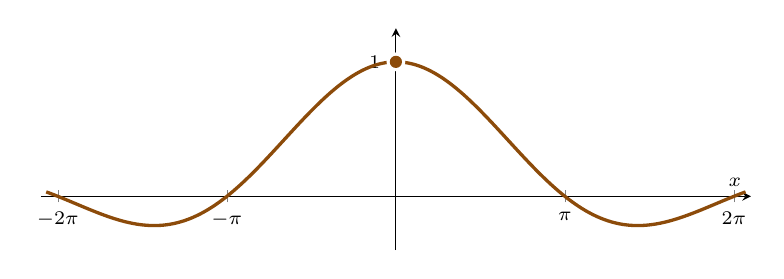
\begin{tikzpicture}
    \begin{axis}[
      width=10.6cm, height=4.4cm,
      axis lines=middle,
      xlabel={$x$}, ylabel={},
      xmin=-6.6, xmax=6.6, ymin=-0.4, ymax=1.25,
      xtick={-6.283,-3.1416,3.1416,6.283},
      xticklabels={$-2\pi$,$-\pi$,$\pi$,$2\pi$},
      ytick={1}, tick label style={font=\scriptsize},
      label style={font=\scriptsize},
    ]
      \addplot[excolor, line width=1.2pt, domain=0.02:6.5, samples=120]
        ({x}, {sin(deg(x))/x});
      \addplot[excolor, line width=1.2pt, domain=-6.5:-0.02, samples=120]
        ({x}, {sin(deg(x))/x});
      \fill[white] (axis cs:0,1) circle (3.4pt);
      \fill[excolor] (axis cs:0,1) circle (2.2pt);
    \end{axis}
  \end{tikzpicture}
  \end{center}

  \note{
    The most famous instance is the limit of sine of "x" over "x" as "x"
    goes to zero. Both the top and the bottom vanish at zero, so it is a
    zero over zero form. Taking the derivative of the top, cosine of "x",
    and of the bottom, one, the quotient of derivatives is cosine of "x"
    over one, which tends to one. So the original limit is one. This also
    matches a familiar geometric fact: for a small angle, the sine of "x" is
    very nearly "x" itself, so their ratio sits close to one. The picture
    shows the graph of sine of "x" over "x" in amber. Away from the origin
    it dips and oscillates, but as "x" approaches zero from either side the
    curve rises smoothly to the height one, marked by the dot on the
    vertical axis. There is no actual spike or hole in the limiting value;
    the function fills in to one. We are borrowing the derivatives of the
    trigonometric functions here, which we will justify in Chapter 8, just
    as the book does. Now let's state the theorem in full generality.
  }
\end{frame}
}

{
\usebackgroundtemplate{%
  
\includegraphics[width=\paperwidth,height=\paperheight,keepaspectratio=false]{chapter_05_bg_02.png}%
}
\section{The Rule}

\begin{frame}{Theorem 5.13: L'Hospital's Rule}
  \begin{thmblock}{Theorem 5.13}
    \small
    Suppose $f$, $g$ are real and differentiable in $(a, b)$, with
    $g'(x) \neq 0$ there and $-\infty \leq a < b \leq +\infty$. If
    \[
      \frac{f'(x)}{g'(x)} \to A \quad (x \to a) \tag{13}
    \]
    and \alert{either}
    \[
      f(x) \to 0,\ \ g(x) \to 0 \quad(14)
      \qquad\text{\alert{or}}\qquad
      g(x) \to +\infty \quad(15)
    \]
    as $x \to a$, then
    \[
      \frac{f(x)}{g(x)} \to A \quad (x \to a). \tag{16}
    \]
  \end{thmblock}

  \note{
    Here is the theorem. Suppose "f" and "g" are differentiable on the open
    interval from "a" to "b", and the derivative of "g" is never zero there.
    The endpoints "a" and "b" are allowed to be infinite, which is why the
    rule handles limits at infinity too. The crucial hypothesis, labeled
    thirteen, is that the quotient of derivatives, "f" prime over "g" prime,
    tends to a limit "A" as "x" approaches "a". Then, provided either
    condition fourteen holds, where both "f" and "g" tend to zero, or
    condition fifteen holds, where "g" tends to plus infinity, the original
    quotient "f" over "g" also tends to the same value "A". The practical
    payoff is that we may trade a hard quotient for the often simpler quotient
    of derivatives, and the one thing we must check is that this derivative
    quotient actually has a limit. So the two indeterminate forms from the
    motivation are covered by one clean statement. Let's read the two cases
    side by side.
  }
\end{frame}

\begin{frame}{Reading the Two Cases}
  \begin{columns}[t]
    \begin{column}{0.48\textwidth}
      \begin{exblock}{Case (14): the $\frac{0}{0}$ form}
        $f \to 0$ and $g \to 0$.
        \[
          \frac{f}{g} \to A
        \]
      \end{exblock}
    \end{column}
    \begin{column}{0.48\textwidth}
      \begin{exblock}{Case (15): the $\frac{\ast}{\infty}$ form}
        $g \to +\infty$
        (the top is \emph{unrestricted}).
        \[
          \frac{f}{g} \to A
        \]
      \end{exblock}
    \end{column}
  \end{columns}

  \vspace{0.6em}
  \begin{hlbox}
  \begin{itemize}
    \item In case (15) we need \alert{nothing} about $f$ --- only that
      $g \to +\infty$
    \item Both cases share the \alert{same} conclusion and the same
      hypothesis (13)
  \end{itemize}
  \end{hlbox}

  \note{
    It is worth pausing on the two cases. On the left is the zero over zero
    form: both "f" and "g" tend to zero, and the conclusion is that their
    ratio tends to "A". On the right is the infinity case: here we only
    require that "g" tends to plus infinity. Notice something surprising
    about the right hand case: we assume nothing whatsoever about the
    numerator "f". It does not have to tend to infinity, or to zero, or to
    anything in particular. The single assumption that the denominator blows
    up, combined with the hypothesis on the quotient of derivatives, is
    enough. Both cases deliver the same conclusion from the same key
    hypothesis, condition thirteen. Let's watch that infinity case in action.
  }
\end{frame}

\begin{frame}[c]{Case (15) in Action: $\dfrac{\log x}{x}$}
  \begin{exblock}{Example (log derivative previewed from Chap.\ 8)}
    As $x \to +\infty$, both $\log x \to +\infty$ and $x \to +\infty$:
    \[
      \lim_{x \to +\infty} \frac{\log x}{x}
        = \lim_{x \to +\infty} \frac{1/x}{1} = 0.
    \]
  \end{exblock}

  \begin{center}
  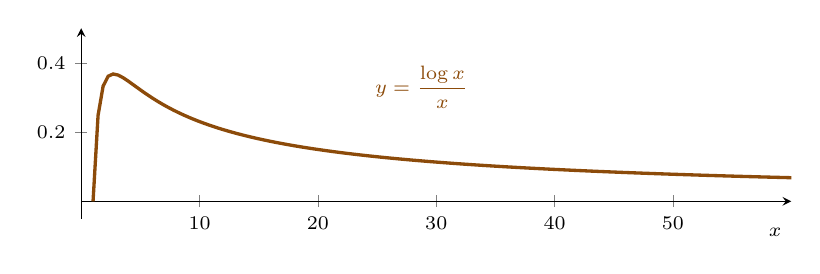
\begin{tikzpicture}
    \begin{axis}[
      width=10.6cm, height=4.0cm,
      axis lines=middle,
      xlabel={$x$}, ylabel={},
      xlabel style={at={(axis description cs:1,0)}, anchor=north east},
      xmin=0, xmax=60, ymin=-0.05, ymax=0.5,
      xtick={10,20,30,40,50}, ytick={0.2,0.4},
      tick label style={font=\scriptsize}, label style={font=\scriptsize},
    ]
      \addplot[excolor, line width=1.2pt, domain=1:60, samples=140]
        ({x}, {ln(x)/x});
      \node[excolor, font=\scriptsize, anchor=west]
        at (axis cs:24,0.33) {$y = \dfrac{\log x}{x}$};
    \end{axis}
  \end{tikzpicture}
  \end{center}

  \note{
    Let's watch the infinity case at work. Take the logarithm of "x" divided
    by "x" as "x" tends to plus infinity. Both the top and the bottom grow
    without bound, so this is the infinity form handled by condition fifteen.
    Differentiating, the top becomes one over "x" and the bottom becomes one,
    so the quotient of derivatives is one over "x", which tends to zero. Hence
    the original quotient tends to zero as well. The amber curve on the slide
    tells the same story: it climbs to a small hump near the left and then
    decays steadily back toward the horizontal axis, showing that "x"
    eventually outruns the logarithm. This is the precise sense in which
    logarithmic growth is slower than linear growth. And notice, in keeping
    with case fifteen, we only needed the denominator to blow up; we placed no
    condition on the numerator. Now a few remarks on the fine print.
  }
\end{frame}

\begin{frame}{Remarks on the Statement}
  \begin{remblock}{Variants and conventions}
    \begin{itemize}
      \item Analogous statements hold as $x \to b$, or if
        $g(x) \to -\infty$ in (15)
      \item Limits are taken in the \alert{extended} sense of
        Definition 4.33, so $A$ may be $\pm\infty$
    \end{itemize}
  \end{remblock}

  \vspace{0.5em}
  \begin{hlbox}
  \textbf{Why $g' \neq 0$ matters:} a derivative has the intermediate value
  property (Theorem 5.12), so $g'$ cannot be positive at one point and
  negative at another without vanishing in between. Hence
  \alert{$g' > 0$ on all of $(a,b)$, \emph{or} $g' < 0$ on all of $(a,b)$} ---
  so $g$ is strictly monotonic and $g(x) - g(y) \neq 0$, keeping every
  denominator in the proof safe.
  \end{hlbox}

  \note{
    A few remarks round out the statement. First, everything we say for the
    limit as "x" approaches the left endpoint "a" has a mirror image for the
    limit as "x" approaches the right endpoint "b"; and the infinity case
    works just as well if "g" tends to minus infinity instead of plus
    infinity. Second, all these limits are understood in the extended sense
    of Definition 4.33 from Chapter 4, which means the target value "A" is
    itself allowed to be plus or minus infinity, not just a finite number.
    Finally, the assumption that "g" prime is never zero is more powerful than
    it first appears. Recall from the previous section that a derivative has
    the intermediate value property, Theorem 5.12. So "g" prime cannot be
    positive at one point of the interval and negative at another, because then
    it would have to pass through zero somewhere in between, which we have
    ruled out. Therefore "g" prime keeps a single sign on the whole interval:
    either it is positive everywhere, or it is negative everywhere. Either way
    "g" is strictly monotonic, so it takes distinct values at distinct points,
    and every denominator we form in the proof is nonzero. With the statement
    understood, let's see the geometry behind it.
  }
\end{frame}
}

{
\usebackgroundtemplate{%
  
\includegraphics[width=\paperwidth,height=\paperheight,keepaspectratio=false]{chapter_05_bg_03.png}%
}
\section{Proof}

\begin{frame}{Proof Strategy: Theorem 5.13}
  \begin{hlbox}
  \textbf{Goal:} Show $f(x)/g(x) \to A$ as $x \to a$.

  \vspace{0.6em}
  \textbf{Approach (squeeze from both sides):}
  \begin{enumerate}
    \item Pick any $q > A$ and an intermediate $r$ with $A < r < q$;
      hypothesis (13) confines $f'/g'$ below $r$ near $a$
    \item The \alert{generalized MVT} (Theorem 5.9) transfers this bound to
      a ratio of \emph{function values}
    \item Feed in case (14) or case (15) to conclude
      $f(x)/g(x) < q$ near $a$
    \item Symmetrically, any $p < A$ gives $p < f(x)/g(x)$ near $a$
    \item Squeeze: $p < f/g < q$ for all $p < A < q$
      $\Rightarrow$ $f/g \to A$
  \end{enumerate}
  \end{hlbox}

  \note{
    Before the formal proof, here is the strategy. The whole argument is a
    two sided squeeze. We show that the quotient "f" over "g" eventually
    lies below every number "q" that is bigger than "A", and, by a
    symmetric argument, that it eventually lies above every number "p"
    smaller than "A". Together these trap the quotient as close to "A" as we
    like. The bridge from the hypothesis on derivatives to a statement about
    the functions themselves is the generalized mean value theorem from
    Section 2. That is the step that makes derivatives talk to function
    values. Steps three and four are where the two cases, zero over zero and
    the infinity case, are actually used. Let's first recall the tool that
    powers step two.
  }
\end{frame}

\begin{frame}[c]{The Engine: Generalized Mean Value Theorem}
  \begin{remblock}{Recall: Theorem 5.9}
    For $a < x < y < c$, there is $t \in (x, y)$ with
    $\dfrac{f(x)-f(y)}{g(x)-g(y)} = \dfrac{f'(t)}{g'(t)}$.
  \end{remblock}

  \begin{center}
  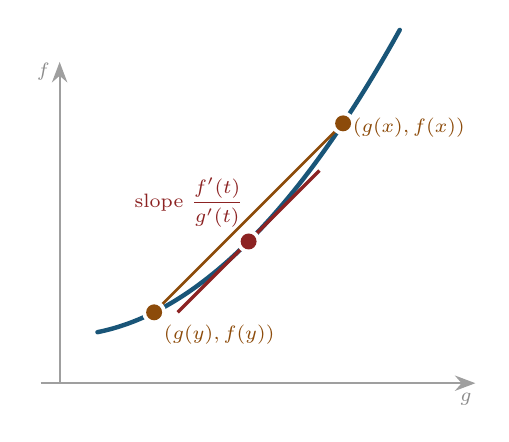
\begin{tikzpicture}[scale=1.2]
    \draw[axisln] (-0.2,-0.5) -- (4.4,-0.5);
    \draw[axisln] (0,-0.5) -- (0,2.9);
    \node[gray!90, below, font=\scriptsize] at (4.3,-0.5) {$g$};
    \node[gray!90, left, font=\scriptsize] at (0,2.8) {$f$};
    % parametric curve (g(t), f(t)) = (u, 0.25 u^2)
    \draw[curveln, defcolor, domain=0.4:3.6, smooth, samples=60]
      plot (\x, {0.25*\x*\x});
    % chord between (1,0.25) and (3,2.25), slope = 1
    \draw[excolor, line width=1pt] (1.0,0.25) -- (3.0,2.25);
    \dotpt{excolor}{(1.0,0.25)}
    \dotpt{excolor}{(3.0,2.25)}
    \node[excolor, right, font=\scriptsize] at (3.0,2.2) {$(g(x),f(x))$};
    \node[excolor, below right, font=\scriptsize] at (1.0,0.22)
      {$(g(y),f(y))$};
    % tangent at (2,1), slope 1, parallel to chord
    \draw[thmcolor, line width=1.2pt] (1.25,0.25) -- (2.75,1.75);
    \dotpt{thmcolor}{(2.0,1.0)}
    \node[thmcolor, above left, font=\scriptsize] at (2.05,1.05)
      {slope $\dfrac{f'(t)}{g'(t)}$};
  \end{tikzpicture}
  \end{center}

  \note{
    The engine of the proof is Theorem 5.9, the generalized mean value
    theorem. It says that for two points "x" and "y", there is some
    intermediate point "t" where the ratio of the differences, "f" of "x"
    minus "f" of "y" over "g" of "x" minus "g" of "y", equals the ratio of
    the derivatives at "t". The picture makes this geometric. Think of the
    pair "g" of "t" and "f" of "t" as tracing a curve in the plane, shown in
    blue. The two amber points are the endpoints, and the amber line joining
    them is the chord; its slope is exactly that ratio of differences.
    Theorem 5.9 promises a point on the curve, marked in red, where the
    tangent line runs parallel to the chord. The slope of that tangent is
    the ratio of the derivatives, "f" prime of "t" over "g" prime of "t".
    Intuitively, the average rate of climb measured across the chord must be
    matched by the instantaneous rate at some point in between. So a bound on
    the derivative ratio becomes a bound on the chord slope. Now we begin the
    proof.
  }
\end{frame}

% --- Build 1/6 ---
\begin{frame}{Proof of Theorem 5.13}
  \begin{proofblock}{Step 1: Confine the derivative ratio}
    Assume $-\infty \leq A < +\infty$. Choose $q$ with $A < q$, then $r$
    with $A < r < q$. By (13) there is $c \in (a, b)$ such that
    \[
      a < x < c \ \Longrightarrow\ \frac{f'(x)}{g'(x)} < r. \tag{17}
    \]
  \end{proofblock}

  \note{
    Step one. We handle the case where "A" is less than plus infinity;
    the other case is symmetric. Fix any number "q" larger than "A", and
    squeeze a second number "r" strictly between "A" and "q". Because the
    quotient of derivatives tends to "A", and "r" is above "A", the quotient
    is eventually below "r". Concretely, there is a cutoff point "c" so that
    for every "x" between "a" and "c", the derivative ratio "f" prime over
    "g" prime is less than "r". This is inequality seventeen. Next we push
    this bound from derivatives onto the functions.
  }
\end{frame}

% --- Build 2/6 ---
\begin{frame}{Proof of Theorem 5.13}
  \begin{proofblock}{Step 2: Apply the generalized MVT}
    If $a < x < y < c$, Theorem 5.9 gives $t \in (x, y)$ with
    \[
      \frac{f(x) - f(y)}{g(x) - g(y)} = \frac{f'(t)}{g'(t)} < r. \tag{18}
    \]
  \end{proofblock}

  \vspace{0.3em}
  \begin{hlbox}
  \textbf{Key step:} the bound (17) on $f'/g'$ now controls a ratio of
  \alert{function values}.
  \end{hlbox}

  \note{
    Step two applies the engine. Take two points "x" and "y" with "x" below
    "y", both to the left of the cutoff "c". The generalized mean value
    theorem gives an intermediate point "t" where the ratio of differences
    equals the derivative ratio there. But "t" lies to the left of "c", so by
    step one that ratio is below "r". This yields inequality eighteen: the
    ratio of the function value differences is less than "r". This is the key
    move of the proof. We began with information about derivatives, and we now
    have a clean inequality about the functions themselves. From here the two
    cases diverge.
  }
\end{frame}

% --- Build 3/6 ---
\begin{frame}{Proof of Theorem 5.13}
  \begin{proofblock}{Step 3: Case (14), the $\frac{0}{0}$ form}
    Fix $y$ and let $x \to a$ in (18). Since $f(x) \to 0$, $g(x) \to 0$:
    \[
      \frac{f(y)}{g(y)} \leq r < q \qquad (a < y < c). \tag{19}
    \]
  \end{proofblock}

  \note{
    Step three treats the zero over zero case, condition fourteen. In
    inequality eighteen, hold "y" fixed and let "x" slide toward the endpoint
    "a". Both "f" of "x" and "g" of "x" go to zero, so the left hand side
    becomes zero minus "f" of "y", over zero minus "g" of "y", which is just
    "f" of "y" over "g" of "y". The strict inequality relaxes to less than or
    equal in the limit, giving inequality nineteen: "f" of "y" over "g" of "y"
    is at most "r", hence below "q", for every "y" between "a" and "c". So the
    quotient is already bounded above by "q". Now the harder infinity case.
  }
\end{frame}

% --- Build 4/6 ---
\begin{frame}{Proof of Theorem 5.13}
  \begin{proofblock}{Step 4: Case (15), the $g \to +\infty$ form}
    Fix $y$; choose $c_1 \in (a, y)$ so that $g(x) > g(y)$ and $g(x) > 0$
    for $a < x < c_1$. Multiply (18) by
    $\dfrac{g(x) - g(y)}{g(x)} > 0$:
    \[
      \frac{f(x)}{g(x)} < r - r\,\frac{g(y)}{g(x)} + \frac{f(y)}{g(x)}
      \qquad (a < x < c_1). \tag{20}
    \]
  \end{proofblock}

  \note{
    Step four is the infinity case, condition fifteen, and it takes a little
    algebra. This time we keep "y" fixed and use that "g" of "x" tends to
    plus infinity. So for "x" close enough to "a", say to the left of a new
    cutoff "c" sub one, the value "g" of "x" is positive and larger than "g"
    of "y". That makes the factor "g" of "x" minus "g" of "y", all over "g"
    of "x", a positive number. Multiplying inequality eighteen by this
    positive factor preserves its direction, and after rearranging we arrive
    at inequality twenty. On the right we now have "r", plus two correction
    terms that both carry a "g" of "x" in the denominator. Watch what those
    correction terms do as "x" approaches "a".
  }
\end{frame}

% --- Build 5/6 ---
\begin{frame}{Proof of Theorem 5.13}
  \begin{proofblock}{Step 4 (continued): let $x \to a$}
    In (20), $y$ is fixed and $g(x) \to +\infty$, so the correction terms
    vanish. Hence there is $c_2 \in (a, c_1)$ with
    \[
      \frac{f(x)}{g(x)} < q \qquad (a < x < c_2). \tag{21}
    \]
  \end{proofblock}

  \vspace{0.3em}
  \begin{hlbox}
  \textbf{Both cases meet here:} (19) and (21) give the same bound
  $\dfrac{f(x)}{g(x)} < q$ near $a$, for \alert{every} $q > A$.
  \end{hlbox}

  \note{
    Continuing step four, look again at inequality twenty. The number "y"
    is fixed, so "f" of "y" and "g" of "y" are constants, while "g" of "x"
    marches off to infinity. Both correction terms therefore shrink to zero,
    and the right hand side approaches "r", which is below "q". So there is a
    still smaller cutoff, "c" sub two, beyond which the quotient "f" of "x"
    over "g" of "x" is less than "q". That is inequality twenty one. Notice
    that both cases have now landed in exactly the same place: whether we are
    in the zero over zero situation or the infinity situation, we have shown
    that for any "q" bigger than "A", the quotient is eventually less than
    "q". Only the lower bound remains.
  }
\end{frame}

% --- Build 6/6 ---
\begin{frame}{Proof of Theorem 5.13}
  \begin{proofblock}{Step 5: Symmetric lower bound and conclusion}
    If $-\infty < A \leq +\infty$, pick $p < A$; the mirror argument yields
    $c_3$ with
    \[
      p < \frac{f(x)}{g(x)} \qquad (a < x < c_3). \tag{22}
    \]
    So for all $p < A < q$, eventually
    $p < \dfrac{f(x)}{g(x)} < q$, hence
    $\boxed{\ \dfrac{f(x)}{g(x)} \to A \ }$ \quad $\blacksquare$
  \end{proofblock}

  \vspace{0.2em}
  \begin{center}
  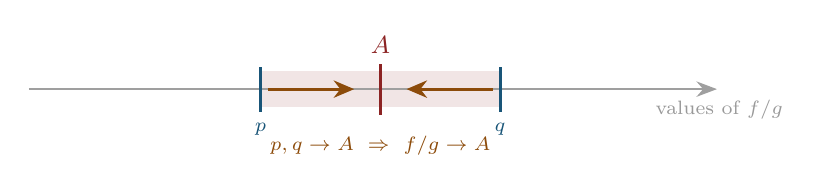
\begin{tikzpicture}[scale=0.95]
    % shaded band (p, q)
    \fill[thmcolor!12] (2.9,-0.24) rectangle (6.1,0.24);
    % number line
    \draw[axisln] (-0.2,0) -- (9.0,0);
    \node[gray!80, font=\scriptsize, below right] at (8.05,-0.02)
      {values of $f/g$};
    % target A at center
    \draw[thmcolor, line width=1.1pt] (4.5,-0.34) -- (4.5,0.34);
    \node[thmcolor, above, font=\small] at (4.5,0.34) {$A$};
    % bounds p and q
    \draw[defcolor, line width=1.1pt] (2.9,-0.3) -- (2.9,0.3);
    \draw[defcolor, line width=1.1pt] (6.1,-0.3) -- (6.1,0.3);
    \node[defcolor, below, font=\scriptsize] at (2.9,-0.32) {$p$};
    \node[defcolor, below, font=\scriptsize] at (6.1,-0.32) {$q$};
    % arrows squeezing inward toward A
    \draw[excolor, guide] (3.0,0) -- (4.15,0);
    \draw[excolor, guide] (6.0,0) -- (4.85,0);
    \node[excolor, font=\scriptsize, below] at (4.5,-0.5)
      {$p, q \to A \ \Rightarrow\ f/g \to A$};
  \end{tikzpicture}
  \end{center}

  \note{
    Step five closes the argument by symmetry. The same reasoning with the
    inequalities reversed shows that for any number "p" below "A", the
    quotient eventually exceeds "p"; that is inequality twenty two. Combining
    this with the upper bound, given any "p" below "A" and any "q" above "A",
    the quotient is eventually caught strictly between them. The number line
    at the bottom pictures exactly this: the target "A" is the red mark in
    the middle, the two blue markers are the bounds "p" and "q", and the
    shaded band is where the quotient finally lands. Since "p" and "q" can be
    pushed as close to "A" as we please, shown by the amber arrows closing
    inward, the quotient must tend to "A", in the extended sense. The proof
    is complete. Let's gather the takeaways.
  }
\end{frame}
}

{
\usebackgroundtemplate{%
  
\includegraphics[width=\paperwidth,height=\paperheight,keepaspectratio=false]{chapter_05_bg_04.png}%
}
\section{Summary}

% --- Build 1/4 ---
\begin{frame}{Summary}
  \begin{hlbox}
  \textbf{Key takeaways from this section:}
  \begin{itemize}
    \item \textbf{Theorem 5.13 (L'Hospital):} if $f'/g' \to A$ and either
      $f, g \to 0$ or $g \to +\infty$, then $f/g \to A$
  \end{itemize}
  \end{hlbox}

  \note{
    Let's review. The star of this section is Theorem 5.13, Lopital's rule.
    Its message is simple to remember: if the quotient of the derivatives
    tends to a limit "A", and if we are in one of the two indeterminate
    situations, either both functions tend to zero, or the denominator tends
    to plus infinity, then the quotient of the original functions tends to
    the same limit "A". This converts a hard limit into an often easier one.
  }
\end{frame}

% --- Build 2/4 ---
\begin{frame}{Summary}
  \begin{hlbox}
  \textbf{Key takeaways from this section:}
  \begin{itemize}
    \item \textbf{Theorem 5.13 (L'Hospital):} if $f'/g' \to A$ and either
      $f, g \to 0$ or $g \to +\infty$, then $f/g \to A$
    \item \textbf{Engine of the proof:} the generalized mean value theorem
      (5.9) turns a derivative bound into a function-value bound
  \end{itemize}
  \end{hlbox}

  \note{
    The proof was not just a formal manipulation; it rested on one central
    idea. The generalized mean value theorem from Section 2 is what lets us
    convert information about the derivatives into information about the
    functions. Everything else was a careful two sided squeeze, trapping the
    quotient between an arbitrary number below "A" and an arbitrary number
    above "A". This pattern, bound the derivative, transfer with the mean
    value theorem, then squeeze, recurs throughout analysis.
  }
\end{frame}

% --- Build 3/4 ---
\begin{frame}{Summary}
  \begin{hlbox}
  \textbf{Key takeaways from this section:}
  \begin{itemize}
    \item \textbf{Theorem 5.13 (L'Hospital):} if $f'/g' \to A$ and either
      $f, g \to 0$ or $g \to +\infty$, then $f/g \to A$
    \item \textbf{Engine of the proof:} the generalized mean value theorem
      (5.9) turns a derivative bound into a function-value bound
    \item \textbf{Generality:} endpoints and $A$ may be $\pm\infty$; the
      $g \to +\infty$ case needs \alert{no} hypothesis on $f$
  \end{itemize}
  \end{hlbox}

  \note{
    A word on how general this really is. The endpoints "a" and "b" are
    allowed to be infinite, so the rule covers limits at infinity, not just
    at finite points. The target "A" may also be infinite. And recall the
    striking feature of the infinity case: when the denominator blows up, we
    need no assumption at all on the numerator. These are not decorations;
    they are what make the theorem so widely applicable. But there is one
    important limitation to flag.
  }
\end{frame}

% --- Build 4/4 ---
\begin{frame}{Summary}
  \begin{hlbox}
  \textbf{Key takeaways from this section:}
  \begin{itemize}
    \item \textbf{Theorem 5.13 (L'Hospital):} if $f'/g' \to A$ and either
      $f, g \to 0$ or $g \to +\infty$, then $f/g \to A$
    \item \textbf{Engine of the proof:} the generalized mean value theorem
      (5.9) turns a derivative bound into a function-value bound
    \item \textbf{Generality:} endpoints and $A$ may be $\pm\infty$; the
      $g \to +\infty$ case needs \alert{no} hypothesis on $f$
    \item \textbf{Warning:} the rule \alert{fails} for complex / vector
      valued functions (Example 5.18)
  \end{itemize}

  \vspace{0.6em}
  \textbf{Coming up next:} Derivatives of Higher Order and Taylor's Theorem.
  \end{hlbox}

  \note{
    The final and most important caveat: Lopital's rule is a theorem about
    real valued functions, and it genuinely breaks down for complex or
    vector valued functions. We will meet a concrete counterexample later in
    the chapter, in Example 5.18, where the quotient of derivatives tends to
    zero but the quotient of the functions does not. The reason traces back
    to the mean value theorem itself, which also fails in that setting. So
    keep the rule in its lane: real functions only. In the next episode we
    turn to derivatives of higher order and build toward Taylor's theorem,
    which approximates a function by a polynomial and estimates the error.
    See you there.
  }
\end{frame}
}

\end{document}
